\documentclass[12pt, fullpage,letterpaper]{article}

\usepackage[margin=1in]{geometry}
\usepackage{url}
\usepackage{amsmath}
\usepackage{amssymb}
\usepackage{xspace}
\usepackage{graphicx}
\usepackage{hyperref}
\usepackage{listings}

\newcommand{\semester}{Spring 2020}
\newcommand{\assignmentId}{2}
\newcommand{\releaseDate}{11 Feb, 2019}
\newcommand{\dueDate}{11:59pm, 25 Feb, 2019}

\newcommand{\bx}{{\bf x}}
\newcommand{\bw}{{\bf w}}

\title{CS 5350/6350: Machine Learining \semester}
\author{Homework \assignmentId}
\date{Handed out: \releaseDate\\
	Due: \dueDate}


\title{CS 5350/6350: Machine Learning \semester}
\author{Homework \assignmentId}
\date{Handed out: \releaseDate\\
  Due date: \dueDate}
\author{Homework \assignmentId \\* Britton Gaul \\* u0915408}
\begin{document}
\maketitle

% Math commands by Thomas Minka
\newcommand{\var}{{\rm var}}
\newcommand{\Tr}{^{\rm T}}
\newcommand{\vtrans}[2]{{#1}^{(#2)}}
\newcommand{\kron}{\otimes}
\newcommand{\schur}[2]{({#1} | {#2})}
\newcommand{\schurdet}[2]{\left| ({#1} | {#2}) \right|}
\newcommand{\had}{\circ}
\newcommand{\diag}{{\rm diag}}
\newcommand{\invdiag}{\diag^{-1}}
\newcommand{\rank}{{\rm rank}}
% careful: ``null'' is already a latex command
\newcommand{\nullsp}{{\rm null}}
\newcommand{\tr}{{\rm tr}}
\renewcommand{\vec}{{\rm vec}}
\newcommand{\vech}{{\rm vech}}
\renewcommand{\det}[1]{\left| #1 \right|}
\newcommand{\pdet}[1]{\left| #1 \right|_{+}}
\newcommand{\pinv}[1]{#1^{+}}
\newcommand{\erf}{{\rm erf}}
\newcommand{\hypergeom}[2]{{}_{#1}F_{#2}}

% boldface characters
\renewcommand{\a}{{\bf a}}
\renewcommand{\b}{{\bf b}}
\renewcommand{\c}{{\bf c}}
\renewcommand{\d}{{\rm d}}  % for derivatives
\newcommand{\e}{{\bf e}}
\newcommand{\f}{{\bf f}}
\newcommand{\g}{{\bf g}}
\newcommand{\h}{{\bf h}}
%\newcommand{\k}{{\bf k}}
% in Latex2e this must be renewcommand
\renewcommand{\k}{{\bf k}}
\newcommand{\m}{{\bf m}}
\newcommand{\mb}{{\bf m}}
\newcommand{\n}{{\bf n}}
\renewcommand{\o}{{\bf o}}
\newcommand{\p}{{\bf p}}
\newcommand{\q}{{\bf q}}
\renewcommand{\r}{{\bf r}}
\newcommand{\s}{{\bf s}}
\renewcommand{\t}{{\bf t}}
\renewcommand{\u}{{\bf u}}
\renewcommand{\v}{{\bf v}}
\newcommand{\w}{{\bf w}}
\newcommand{\x}{{\bf x}}
\newcommand{\y}{{\bf y}}
\newcommand{\z}{{\bf z}}
%s\newcommand{\l}{\boldsymbol{l}}
\newcommand{\A}{{\bf A}}
\newcommand{\B}{{\bf B}}
\newcommand{\C}{{\bf C}}
\newcommand{\D}{{\bf D}}
\newcommand{\E}{{\bf E}}
\newcommand{\F}{{\bf F}}
\newcommand{\G}{{\bf G}}
\renewcommand{\H}{{\bf H}}
\newcommand{\I}{{\bf I}}
\newcommand{\J}{{\bf J}}
\newcommand{\K}{{\bf K}}
\renewcommand{\L}{{\bf L}}
\newcommand{\M}{{\bf M}}
\newcommand{\N}{\mathcal{N}}  % for normal density
%\newcommand{\N}{{\bf N}}
\renewcommand{\O}{{\bf O}}
\renewcommand{\P}{{\bf P}}
\newcommand{\Q}{{\bf Q}}
\newcommand{\R}{{\bf R}}
\renewcommand{\S}{{\bf S}}
\newcommand{\T}{{\bf T}}
\newcommand{\U}{{\bf U}}
\newcommand{\V}{{\bf V}}
\newcommand{\W}{{\bf W}}
\newcommand{\X}{{\bf X}}
\newcommand{\Y}{{\bf Y}}
\newcommand{\Z}{{\bf Z}}

% this is for latex 2.09
% unfortunately, the result is slanted - use Latex2e instead
%\newcommand{\bfLambda}{\mbox{\boldmath$\Lambda$}}
% this is for Latex2e
\newcommand{\bfLambda}{\boldsymbol{\Lambda}}

% Yuan Qi's boldsymbol
\newcommand{\bsigma}{\boldsymbol{\sigma}}
\newcommand{\balpha}{\boldsymbol{\alpha}}
\newcommand{\bpsi}{\boldsymbol{\psi}}
\newcommand{\bphi}{\boldsymbol{\phi}}
\newcommand{\boldeta}{\boldsymbol{\eta}}
\newcommand{\Beta}{\boldsymbol{\eta}}
\newcommand{\btau}{\boldsymbol{\tau}}
\newcommand{\bvarphi}{\boldsymbol{\varphi}}
\newcommand{\bzeta}{\boldsymbol{\zeta}}

\newcommand{\blambda}{\boldsymbol{\lambda}}
\newcommand{\bLambda}{\mathbf{\Lambda}}
\newcommand{\bOmega}{\mathbf{\Omega}}
\newcommand{\bomega}{\mathbf{\omega}}
\newcommand{\bPi}{\mathbf{\Pi}}

\newcommand{\btheta}{\boldsymbol{\theta}}
\newcommand{\bpi}{\boldsymbol{\pi}}
\newcommand{\bxi}{\boldsymbol{\xi}}
\newcommand{\bSigma}{\boldsymbol{\Sigma}}

\newcommand{\bgamma}{\boldsymbol{\gamma}}
\newcommand{\bGamma}{\mathbf{\Gamma}}

\newcommand{\bmu}{\boldsymbol{\mu}}
\newcommand{\1}{{\bf 1}}
\newcommand{\0}{{\bf 0}}

% \newcommand{\comment}[1]{}

\newcommand{\bs}{\backslash}
\newcommand{\ben}{\begin{enumerate}}
\newcommand{\een}{\end{enumerate}}

 \newcommand{\notS}{{\backslash S}}
 \newcommand{\nots}{{\backslash s}}
 \newcommand{\noti}{{\backslash i}}
 \newcommand{\notj}{{\backslash j}}
 \newcommand{\nott}{\backslash t}
 \newcommand{\notone}{{\backslash 1}}
 \newcommand{\nottp}{\backslash t+1}
% \newcommand{\notz}{\backslash z}

\newcommand{\notk}{{^{\backslash k}}}
%\newcommand{\noti}{{^{\backslash i}}}
\newcommand{\notij}{{^{\backslash i,j}}}
\newcommand{\notg}{{^{\backslash g}}}
\newcommand{\wnoti}{{_{\w}^{\backslash i}}}
\newcommand{\wnotg}{{_{\w}^{\backslash g}}}
\newcommand{\vnotij}{{_{\v}^{\backslash i,j}}}
\newcommand{\vnotg}{{_{\v}^{\backslash g}}}
\newcommand{\half}{\frac{1}{2}}
\newcommand{\msgb}{m_{t \leftarrow t+1}}
\newcommand{\msgf}{m_{t \rightarrow t+1}}
\newcommand{\msgfp}{m_{t-1 \rightarrow t}}

\newcommand{\proj}[1]{{\rm proj}\negmedspace\left[#1\right]}
\newcommand{\argmin}{\operatornamewithlimits{argmin}}
\newcommand{\argmax}{\operatornamewithlimits{argmax}}

\newcommand{\dif}{\mathrm{d}}
\newcommand{\abs}[1]{\lvert#1\rvert}
\newcommand{\norm}[1]{\lVert#1\rVert}

%miscellaneous symbols
\newcommand{\ie}{{{i.e.,}}\xspace}
\newcommand{\eg}{{{\em e.g.,}}\xspace}
\newcommand{\EE}{\mathbb{E}}
\newcommand{\VV}{\mathbb{V}}
\newcommand{\sbr}[1]{\left[#1\right]}
\newcommand{\rbr}[1]{\left(#1\right)}
\newcommand{\cmt}[1]{}




\section{Paper Problems [40 points + 8 bonus]}
\begin{enumerate}
\item~

\begin{enumerate}
	\item~
	\begin{enumerate}
		\item~
		\newline According to Occam's Razor $H_2$ should be chosen for the result hypothesis. This is because both of the result hypothesises are consistent with the training data, but $H_2$ is smaller than $H$.
		\item~
		\newline This prinicple is reflected in the PAC guarantee, because the samller hypothesis that was chosen is more likely to be less then the total number of m examples. This is required because it is stated in the given equation. 
	\end{enumerate}
	\item~
	\newline $3^{10} \cdot .90 = 53,145$ training examples needed. 
\end{enumerate}

\item~

\item~
	\begin{enumerate}
		\item~ 
		\newline $x_1 - x_2-x_3 \geq 2 $
		\item~
		\newline $-x_1-x_2-x_3 \geq -1$
		\item~
		\newline $x_1+x_2+x_3+x_4 \geq 2$
		\item ~
		\newline $x_1+x_2-x_1+x_2 \geq 1$
	\end{enumerate}
		
	
	\item

\item~  

\begin{enumerate}
	\item~
	\newline $j(w, b)=\frac{1}{2} \sum_{n=1}^{m} (y_i - w^Tx_i)^2 \cdot b$ 
	\item~
	\item~
	\item~  
\end{enumerate}
\end{enumerate}

\section{Practice [60 points + 10 bonus]}
\begin{enumerate}
	\item~[2 Points]  
	\newline Repository: https://github.com/BritGaul/CS5350

\item~
\begin{enumerate}
	\item~
	\newline 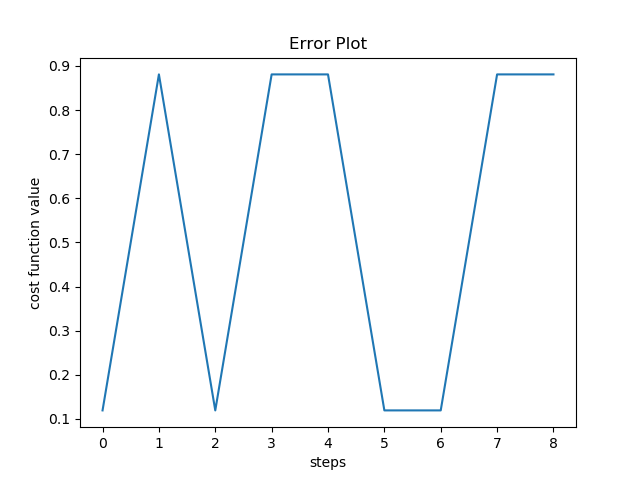
\includegraphics{prob_2_2_a.png}
	\newline When using the Adaboost decision trees the errors are smaller compared to a fully expanded decsion tree, which makes them more accurate. 
	
	\item~
	\newline Overall the bagged trees seem to be better than a single tree. However, when compared to the Addaboost trees it seems that the adaboosted trees are more accurate. 

	\item~ 
	\newline When comparing the results from the single tree learner verses the bagged trees, the bagged trees are more accurate. This is because the bagged trees can learn from the accuracies of previous trees, while the single tree has no other trees to learn from. 
	 
	\item~ 
	\newline The random forrest algorithm runs more efficiently then the bagged trees alogorithm, but is less accurate then the bagged trees implementation. 
	
\end{enumerate}

	\item~
	
	\begin{enumerate}
		\item~
		\newline Learned weight vector: [0.92121924, 0.80795412, 0.87360641, 1.31402335, 0.13386879, 1.59860304, 1.01995499]
		\newline Learning Rate: 0.0125
		\newline 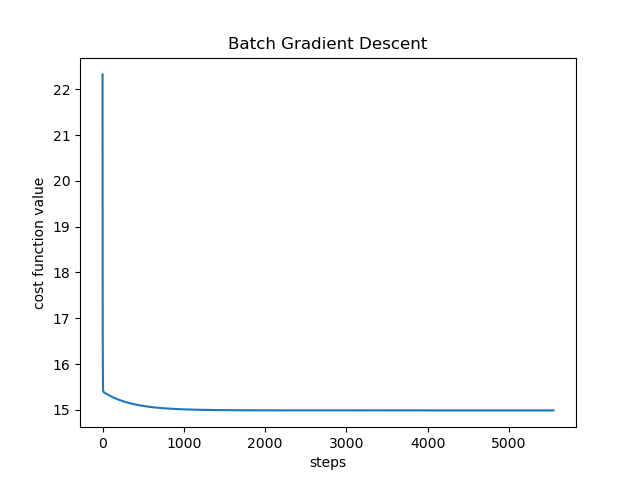
\includegraphics{gradient_descent.png}
		\item~
		\newline Learned weight vector: [0.72954178 0.60583116, 0.65623542, 1.16051283, 0.10111029, 1.33361719, 0.8242626 ]
		\newline Learning Rate: 0.001
		\newline 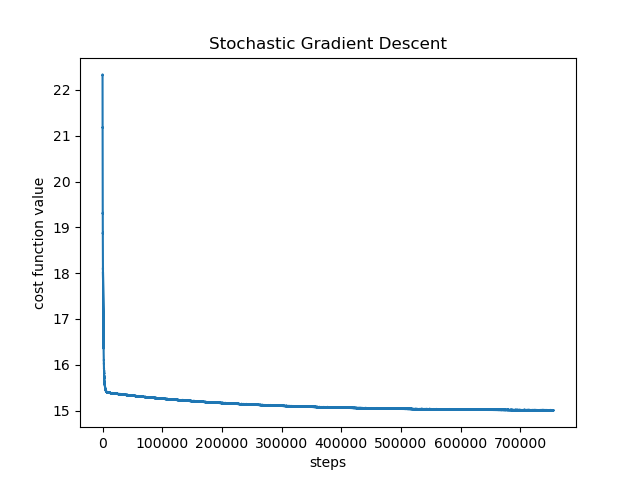
\includegraphics{stochastic_gradient.png}
		\item~
		\newline Learned weight vector: [0.92154947, 0.80829428, 0.87397433, 1.3142877,  0.13392374, 1.59904727, 1.02029192]
		\newline The learned weight vector calcualted with an analytical form is very similar to the weight vector from the batch gradient descent method. By comparing all three weight vectors it seems that the stochastic gradient descent weight vector consistently returns the lowest weights. 
		This could be because the other two methods will always return around the same numbers, where the stochastic approach could get lucky and find the most optimal result randomly. 
	\end{enumerate}

\end{enumerate}

\end{document}
%%% Local Variables:
%%% mode: latex
%%% TeX-master: t
%%% End:
